\documentclass{article}
\usepackage{titling} % Personnalisation du titre
\usepackage[left=20mm, right=20mm]{geometry}
\usepackage{amsmath,amssymb,mathtools}
\usepackage{esint} % intégrale avec un round
\usepackage{xcolor}
\usepackage[utf8]{inputenc}
\usepackage{listings}
\usepackage{enumitem}
\usepackage{multicol}
\usepackage{stmaryrd}
\usepackage{graphicx}
\graphicspath{ {./images/} }
\usepackage[framemethod=tikz]{mdframed}
\usepackage{tikz,pgfplots}
\pgfplotsset{compat=1.18}
\usetikzlibrary{arrows}
\usepackage{forest}
\usepackage{titlesec}
\setlength{\parindent}{0pt}

\pretitle{\begin{center}\Huge\bfseries}
\posttitle{\end{center}}
\date{}
\renewcommand{\thesection}{\Roman{section}} 
\titleformat{\section}
  {\Large\bfseries} % Style du titre
  {\thesection} % Numéro de section
  {0.5cm} % Espacement entre numéro et titre
  {} % Pas de préfixe supplémentaire
\titleformat{\subsection}
  {\large\bfseries} % Style du titre
  {\thesubsection} % Numéro de section
  {0.4cm} % Espacement entre numéro et titre
  {} % Pas de préfixe supplémentair


\newenvironment{enumeratebf}{
    \begin{enumerate}[label=\textbf{\arabic*.}]
}
{
    \end{enumerate}
}
  
\definecolor{oranges}{RGB}{255, 242, 230}
\definecolor{rouges}{RGB}{255, 230, 230}
\definecolor{rose}{RGB}{255, 204, 204}

% maths - info
\definecolor{rouge_fonce}{RGB}{204, 0, 0}
\definecolor{rouge}{RGB}{255, 0, 0}
\definecolor{bleufonce}{RGB}{0, 0, 255}
\definecolor{vert_fonce}{RGB}{0, 69, 33}
\definecolor{vert}{RGB}{0,255,0}

\definecolor{orange_foncee}{RGB}{255, 153, 0}
\definecolor{myrtille}{RGB}{225, 225, 255}
\definecolor{mayonnaise}{RGB}{255, 253, 233}
\definecolor{magenta}{RGB}{224, 209, 240}
\definecolor{pomme}{RGB}{204, 255, 204}
\definecolor{mauve}{RGB}{255, 230, 255}


% Cours

\newmdenv[
    nobreak=true,
    topline=true,
    bottomline=true,
    rightline=true,
    leftline=true,
    linewidth=0.5pt,
    linecolor=black,
    backgroundcolor=mayonnaise,
    innerleftmargin=10pt,
    innerrightmargin=2.5em,
    innertopmargin=5pt,
    innerbottommargin=5pt,
    skipabove=\topsep,
    skipbelow=\topsep,
]{boite_definition}

\newcounter{boite}
\setcounter{boite}{1}
\newenvironment{definition}[2]
{
    \vspace{15pt}
    \begin{boite_definition}
    \if\relax\detokenize{#1}\relax
        \textbf{\textcolor{rouge}{Définition \arabic{chapitre}.\arabic{boite}}}%
        \if\relax\detokenize{#2}\relax
        \else
            \textit{ - #2}
        \fi
        \stepcounter{boite}
    \else
        \textbf{\textcolor{rouge}{Définition #1}}%
        \if\relax\detokenize{#2}\relax
        \else
            \textit{ - #2}
        \fi
    \fi \\
    
    
}
{
    \end{boite_definition}
    \vspace{10pt}
}

\newmdenv[
  nobreak=true,
  topline=true,
  bottomline=true,
  rightline=true,
  leftline=true,
  linewidth=0.5pt,
  linecolor=white,
  backgroundcolor=white,
  innerleftmargin=10pt,
  innerrightmargin=2.5em,
  innertopmargin=5pt,
  innerbottommargin=5pt,
  skipabove=\topsep,
  skipbelow=\topsep,
]{boite_exemple}


\newenvironment{exemple}[2]
{
    \vspace{15pt}
    \begin{boite_exemple}
    \if\relax\detokenize{#1}\relax
        \textbf{\textcolor{bleufonce}{Exemple \arabic{chapitre}.\arabic{boite}}}%
        \if\relax\detokenize{#2}\relax
        \else
            \textit{ - #2}
        \fi
        \stepcounter{boite}
    \else
        \textbf{\textcolor{bleufonce}{Exemple #1}}%
        \if\relax\detokenize{#2}\relax
        \else
            \textit{ - #2}
        \fi
    \fi \\
    
    
}
{
    \end{boite_exemple}
    \vspace{10pt}
}

\newmdenv[
  nobreak=true,
  topline=true,
  bottomline=true,
  rightline=true,
  leftline=true,
  linewidth=0.5pt,
  linecolor=black,
  backgroundcolor=magenta,
  innerleftmargin=10pt,
  innerrightmargin=2.5em,
  innertopmargin=5pt,
  innerbottommargin=5pt,
  skipabove=\topsep,
  skipbelow=\topsep,
]{boite_proposition}

\newenvironment{proposition}[2]
{
    \vspace{15pt}
    \begin{boite_proposition}
    \if\relax\detokenize{#1}\relax
        \textbf{\textcolor{rouge}{Proposition \arabic{chapitre}.\arabic{boite}}}%
        \if\relax\detokenize{#2}\relax
        \else
            \textit{ - #2}
        \fi
        \stepcounter{boite}
    \else
        \textbf{\textcolor{rouge}{Proposition #1}}%
        \if\relax\detokenize{#2}\relax
        \else
            \textit{ - #2}
        \fi
    \fi \\
    
    
}
{
    \end{boite_proposition}
}

\newmdenv[
  nobreak=true,
  topline=true,
  bottomline=true,
  rightline=true,
  leftline=true,
  linewidth=0.5pt,
  linecolor=black,
  backgroundcolor=magenta,
  innerleftmargin=10pt,
  innerrightmargin=2.5em,
  innertopmargin=5pt,
  innerbottommargin=5pt,
  skipabove=\topsep,
  skipbelow=\topsep,
]{boite_theoreme}


\newenvironment{theoreme}[2]
{
    \vspace{15pt}
    \begin{boite_theoreme}
    \if\relax\detokenize{#1}\relax
        \textbf{\textcolor{rouge}{Théorème \arabic{chapitre}.\arabic{boite}}}%
        \if\relax\detokenize{#2}\relax
        \else
            \textit{ - #2}
        \fi
        \stepcounter{boite}
    \else
        \textbf{\textcolor{rouge}{Théorème #1}}%
        \if\relax\detokenize{#2}\relax
        \else
            \textit{ - #2}
        \fi
    \fi \\
    
    
}
{
    \end{boite_theoreme}
}


\newmdenv[
  nobreak=true,
  topline=true,
  bottomline=true,
  rightline=true,
  leftline=true,
  linewidth=0.5pt,
  linecolor=black,
  backgroundcolor=white,
  innerleftmargin=10pt,
  innerrightmargin=2.5em,
  innertopmargin=5pt,
  innerbottommargin=5pt,
  skipabove=\topsep,
  skipbelow=\topsep,
]{boite_demonstration}


\newenvironment{demonstration}
{
    \vspace{15pt}
    \begin{boite_demonstration}
    \textbf{\textcolor{rouge}{Démonstration}}\\ \\
}
{
    \end{boite_demonstration}
    
}


\newmdenv[
  nobreak=true,
  topline=true,
  bottomline=true,
  rightline=true,
  leftline=true,
  linewidth=0.5pt,
  linecolor=white,
  backgroundcolor=white,
  innerleftmargin=10pt,
  innerrightmargin=2.5em,
  innertopmargin=5pt,
  innerbottommargin=5pt,
  skipabove=\topsep,
  skipbelow=\topsep,
]{boite_remarque}


\newenvironment{remarque}[2]
{
    \vspace{15pt}
    \begin{boite_remarque}
    \if\relax\detokenize{#1}\relax
        \textbf{\textcolor{bleufonce}{Remarque \arabic{chapitre}.\arabic{boite}}}%
        \if\relax\detokenize{#2}\relax
        \else
            \textit{ - #2}
        \fi
        \stepcounter{boite}
    \else
        \textbf{\textcolor{bleufonce}{Remarque #1}}%
        \if\relax\detokenize{#2}\relax
        \else
            \textit{ - #2}
        \fi
    \fi \\
    
    
}
{
    \end{boite_remarque}
}

\newmdenv[
  nobreak=true,
  topline=true,
  bottomline=true,
  rightline=true,
  leftline=true,
  linewidth=0.5pt,
  linecolor=bleufonce,
  backgroundcolor=white,
  innerleftmargin=10pt,
  innerrightmargin=2.5em,
  innertopmargin=5pt,
  innerbottommargin=5pt,
  skipabove=\topsep,
  skipbelow=\topsep,
]{boite_implementation}


\definecolor{keywordcolor}{RGB}{133, 153, 0}  % les mots-clés
\definecolor{commentcolor}{RGB}{147, 161, 161} % les commentaires
\definecolor{stringcolor}{RGB}{42, 161, 152}  % les chaînes de caractères

\lstnewenvironment{lstOCaml}
{\lstset{
    language=[Objective]Caml,
    basicstyle=\ttfamily,
    keywordstyle=\color{keywordcolor},
    commentstyle=\color{commentcolor},
    stringstyle=\color{stringcolor},
    backgroundcolor=\color{white},
    numbers=left,
    numberstyle=\ttfamily,
    numbersep=-1.5em,
    stepnumber=1,
    frame=l,
    framexleftmargin=-2.25em,
    tabsize=2,
    literate=%
    {é}{{\'e}}{1}%
    {è}{{\`e}}{1}%
    {à}{{\`a}}{1}%
    {ç}{{\c{c}}}{1}%
    {œ}{{\oe}}{1}%
    {ù}{{\`u}}{1}%
    {É}{{\'E}}{1}%
    {È}{{\`E}}{1}%
    {À}{{\`A}}{1}%
    {Ç}{{\c{C}}}{1}%
    {Œ}{{\OE}}{1}%
    {Ê}{{\^E}}{1}%
    {ê}{{\^e}}{1}%
    {î}{{\^i}}{1}%
    {ô}{{\^o}}{1}%
    {û}{{\^u}}{1}%
    {ä}{{\"{a}}}1
    {ë}{{\"{e}}}1
    {ï}{{\"{i}}}1
    {ö}{{\"{o}}}1
    {ü}{{\"{u}}}1
    {û}{{\^{u}}}1
    {â}{{\^{a}}}1
    {Â}{{\^{A}}}1
    {Î}{{\^{I}}}1
}}{}
 
\lstnewenvironment{lstC}
{\lstset{
    language=C,
    basicstyle=\ttfamily,
    keywordstyle=\color{keywordcolor},
    commentstyle=\color{commentcolor},
    stringstyle=\color{stringcolor},
    backgroundcolor=\color{white},
    numbers=left,
    numberstyle=\ttfamily,
    numbersep=-1.5em,
    stepnumber=1,
    frame=l,
    framexleftmargin=-2.25em,
    tabsize=2,
    literate=%
    {é}{{\'e}}{1}%
    {è}{{\`e}}{1}%
    {à}{{\`a}}{1}%
    {ç}{{\c{c}}}{1}%
    {œ}{{\oe}}{1}%
    {ù}{{\`u}}{1}%
    {É}{{\'E}}{1}%
    {È}{{\`E}}{1}%
    {À}{{\`A}}{1}%
    {Ç}{{\c{C}}}{1}%
    {Œ}{{\OE}}{1}%
    {Ê}{{\^E}}{1}%
    {ê}{{\^e}}{1}%
    {î}{{\^i}}{1}%
    {ô}{{\^o}}{1}%
    {û}{{\^u}}{1}%
    {ä}{{\"{a}}}1
    {ë}{{\"{e}}}1
    {ï}{{\"{i}}}1
    {ö}{{\"{o}}}1
    {ü}{{\"{u}}}1
    {û}{{\^{u}}}1
    {â}{{\^{a}}}1
    {Â}{{\^{A}}}1
    {Î}{{\^{I}}}1
}}{}


\lstdefinelanguage{LNat}{
    morekeywords={tant,que,pour,tout,si,sinon,initialiser,renvoyer,attendre la fin, afficher},
    sensitive=false,
    morecomment=[l]{//},
}

\lstnewenvironment{lstLNat}
{\lstset{
    language=LNat,
    basicstyle=\ttfamily,
    keywordstyle=\color{keywordcolor},
    commentstyle=\color{commentcolor},
    stringstyle=\color{stringcolor},
    backgroundcolor=\color{white},
    numbers=left,
    numberstyle=\ttfamily,
    numbersep=-1.5em,
    stepnumber=1,
    frame=l,
    mathescape=true,
    framexleftmargin=-2.25em,
    tabsize=2,
    literate=%
    {é}{{\'e}}{1}%
    {è}{{\`e}}{1}%
    {à}{{\`a}}{1}%
    {ç}{{\c{c}}}{1}%
    {œ}{{\oe}}{1}%
    {ù}{{\`u}}{1}%
    {É}{{\'E}}{1}%
    {È}{{\`E}}{1}%
    {À}{{\`A}}{1}%
    {Ç}{{\c{C}}}{1}%
    {Œ}{{\OE}}{1}%
    {Ê}{{\^E}}{1}%
    {ê}{{\^e}}{1}%
    {î}{{\^i}}{1}%
    {ô}{{\^o}}{1}%
    {û}{{\^u}}{1}%
    {ä}{{\"{a}}}1
    {ë}{{\"{e}}}1
    {ï}{{\"{i}}}1
    {ö}{{\"{o}}}1
    {ü}{{\"{u}}}1
    {û}{{\^{u}}}1
    {â}{{\^{a}}}1
    {Â}{{\^{A}}}1
    {Î}{{\^{I}}}1}
}{}

\newenvironment{implementation}[1]
{   
    \vspace{15pt}
    \begin{boite_implementation}
    \textbf{\textcolor{bleufonce}{Implémentation}}\textit{ - #1}
     \\ \\
}
{    
    \end{boite_implementation}
}

\newmdenv[
  nobreak=true,
  topline=true,
  bottomline=true,
  rightline=true,
  leftline=true,
  linewidth=0.5pt,
  linecolor=black,
  backgroundcolor=mayonnaise,
  innerleftmargin=10pt,
  innerrightmargin=2.5em,
  innertopmargin=5pt,
  innerbottommargin=5pt,
  skipabove=\topsep,
  skipbelow=\topsep,
]{boite_question}


\newenvironment{question}[2]
{
    \vspace{15pt}
    \begin{boite_question}
    \if\relax\detokenize{#1}\relax
        \textbf{\textcolor{rouge}{Question \arabic{chapitre}.\arabic{boite}}}%
        \if\relax\detokenize{#2}\relax
        \else
            \textit{ - #2}
        \fi
        \stepcounter{boite}
    \else
        \textbf{\textcolor{rouge}{Question #1}}%
        \if\relax\detokenize{#2}\relax
        \else
            \textit{ - #2}
        \fi
    \fi \\
    
    
}
{
    \end{boite_question}
}

\newmdenv[
  nobreak=true,
  topline=true,
  bottomline=true,
  rightline=true,
  leftline=true,
  linewidth=0.5pt,
  linecolor=black,
  backgroundcolor=white,
  innerleftmargin=10pt,
  innerrightmargin=2.5em,
  innertopmargin=5pt,
  innerbottommargin=5pt,
  skipabove=\topsep,
  skipbelow=\topsep,
]{boite_corollaire}



\newenvironment{corollaire}[2]
{
    \vspace{15pt}
    \begin{boite_corollaire}
    \if\relax\detokenize{#1}\relax
        \textbf{\textcolor{rouge}{Corollaire \arabic{chapitre}.\arabic{boite}}}%
        \if\relax\detokenize{#2}\relax
        \else
            \textit{ - #2}
        \fi
        \stepcounter{boite}
    \else
        \textbf{\textcolor{rouge}{Corollaire #1}}%
        \if\relax\detokenize{#2}\relax
        \else
            \textit{ - #2}
        \fi
    \fi \\
    
    
}
{
    \end{boite_corollaire}
}


\newcounter{chapitre}
\setcounter{chapitre}{11}

\title{\Large Chapitre 11 \\ \Huge Classes de complexité}

\begin{document}
% commandes
\newcommand{\notion}[1]{\textcolor{vert_fonce}{\textit{#1}}}
\newcommand{\mb}[1]{\mathbb{#1}}
\newcommand{\mc}[1]{\mathcal{#1}}
\newcommand{\code}[1]{\texttt{#1}}
\newcommand{\ccode}[1]{\texttt{|#1|}}
\newcommand{\ov}[1]{\overline{#1}}
\newcommand{\abs}[1]{|#1|}
\newcommand{\rev}[1]{\texttt{reverse(#1)}}
\newcommand{\crev}[1]{\texttt{|reverse(#1)|}}

\newcommand{\ie}{\textit{i.e.} }

\newcommand{\N}{\mathbb{N}}
\newcommand{\R}{\mathbb{R}}
\newcommand{\C}{\mathbb{C}}
\newcommand{\K}{\mathbb{K}}

\newcommand{\A}{\mathcal{A}}
\newcommand{\bigO}{\mathcal{O}}
\renewcommand{\L}{\mathcal{L}}

\newcommand{\rg}[0]{\text{rg}}
\newcommand{\re}[0]{\text{Re}}
\newcommand{\im}[0]{\text{Im}}
\newcommand{\cl}[0]{\text{cl}}
\newcommand{\mat}[1]{\text{Mat}_{#1}}
\newcommand{\matrice}[1]{\mathcal{M}_{#1}}
\newcommand{\sgEngendre}[1]{\left\langle #1 \right\rangle}
\newcommand{\norme}[1]{||#1||}
\renewcommand{\d}[1]{\,\text{d}#1}
\newcommand{\intint}[2]{\llbracket #1 ,\, #2 \rrbracket}
\newcommand{\seg}[2]{[#1\, ; \, #2]}
\newcommand{\scal}[2]{\left\langle #1 ,\, #2 \right\rangle}
\newcommand{\inte}[2]{\int_{#1}^{#2}}
\newcommand{\somme}[2]{\sum_{#1}^{#2}}





\maketitle


\section{Classes de complexité pour un problème de décision}
\subsection{Complexité}

\newcommand{\pbm}{\mc{P}}
\newcommand{\algo}{\mc{A}}
\newcommand{\reductibleP}{\leq_m^\mr{P}}
\newcommand{\troissat}{\textbf{3-SAT}\,}
\newcommand{\deuxsat}{\textbf{2-SAT}\,}
\newcommand{\cnfsat}{\textbf{CNF-SAT}\,}
\newcommand{\sat}{\textbf{SAT}\,}
\newcommand{\cheminham}{\textbf{CHEMIN-HAM}\,}
\newcommand{\cycleham}{\textbf{CYCLE-HAM}\,}


\begin{definition}{}{}
    Soit $\mc{P}$ un problème abstrait défini par une fonction $f:I\to S$. On considère un algorithme $\mc{A}$ "abstrait" qui le résout.\\
    On y associe un problème \notion{concret} en imposant des choix sur \notion{l'encodage} des entrées et des sorties.\\
    La \notion{complexité du problème concret} correspond à la complexité de l'implémentation de l'algorithme $\algo$ (sa réalisation concrète) pour le choix d'encodage.\\
    C'est-à-dire un ordre de grandeur du nombre d'opérations élémentaires réalisées par l'implémentation de l'algorithme pour une entrée en fonction de la \notion{taille de l'entrée} (espace occupé en mémoire pour son encodage).
\end{definition}

\begin{remarque}{}{cas du graphe}
    La taille de l'encodage pour un graphe~:
    \begin{itemize}
        \item matrice d'adjacence~: $\mc{O}(\abs{S}^2)$
        \item liste d'adjacence~: $\mc{O}(\abs{S} + \abs{A})$
    \end{itemize}
\end{remarque}

\begin{exemple}{}{taille de l'endage des entiers}
    Un entier $n$ s'encode en $\mc{O}(\log_2(n))$, taille de l'écriture binaire.\\
    Une complexité en $\mc{O}(n)$ où $n$ est l'entier en entrée, est donc exponentielle pour un algorithme dont l'entrée est $n$, est $\mc{O}(n) = \mc{O}(2^{\log_2(n)})$. C'est donc exponentiel en la taille de l'entrée !
\end{exemple}

\begin{remarque}{}{relative aux problèmes}
    Selon l'importance des entiers dans le problème, on peut "ignorer" que les entier prennent beaucoup de place~:
    \begin{itemize}
        \item pour un graphe pondéré, la taille des entiers est ignorée.
        \item pour le problème du sac à dos, la taille des entiers est prise en compte.
    \end{itemize}
\end{remarque}

\begin{exemple}{}{}
    \begin{itemize}
        \item \textbf{Instance} : un entier $n$
        \item \textbf{Question} : $v_2(n) \geq v_3(n)$ ? (en parlant de valuation $2$-adique)
    \end{itemize}
    \begin{lstLNat}
    Algo($n$):
        tmp = $n$
        tant que tmp%2 == 0 ou tmp%3==0:
            si tmp%6==0:
                tmp = tmp/6
            sinon si tmp%2==0:
                renvoyer Vrai
            sinon si tmp%3==0:
                renvoyer Faux
        renvoyer Vrai // $v_2(n) = v_3(n)$
    \end{lstLNat}
    La complexité temporelle est en $\mc{O}(\log_6(n)) = \mc{O}(\log_2(n)) = \mc{O}(\abs{n})$. C'est une complexité linéaire en la taille de l'entrée~: $\abs{n} = \log_2(n)$.\\\\
    Moralité : toujours se ramener à une complexité en fonction de la taille de l'entrée.
\end{exemple}

\begin{remarque}{}{}
    La taille de l'entrée est à rapprocher de la taille du mot de $\Sigma = \{0;1\}$ que l'on écrit initialement sur une machine de Turing exécutant l'algorithme sur ce mot.
\end{remarque}

\subsection{Classe P}

\begin{definition}{}{classe P}
    On appelle \notion{classe P} (ou \notion{classe PTIME}) l'ensemble de \notion{problèmes de décision} que l'on peut résoudre à l'aide d'un algorithme de complexité polynomiale en la taille de l'entrée (pour un choix d'encodage).
\end{definition}

\begin{remarque}{}{}
    Généralement, on donne la complexité sous la forme $\mc{O}(\abs{e}^k)$ avec $k$ un entier (degré de l'expression polynomiale de la complexité) et $\abs{e}$ désignant la taille de l'entier.
\end{remarque}

\begin{remarque}{}{}
    Les problèmes de la classe P sont raisonnablement traitables. (Attention, on parle toujours uniquement de problème de décision).\\
    Pour considérer des problèmes d'optimisation, on se ramène à des problèmes de décision en introduisant un seuil à dépasser pour la fonction de coût.
\end{remarque}

\begin{remarque}{}{classe EXP}
    La \notion{classe EXP} (ou \notion{classe EXPTIME}) est la classe de problèmes de décision pour lesquels il existe un algorithme de résolution de complexité exponentielle~:
    $$\mc{O}\Big(P(\abs{e})\exp(\abs{e})\Big)$$
    où $P$ est un polynôme réel et $\abs{e}$ est la taille de l'entrée.
\end{remarque}

\begin{remarque}{}{comparaison entre EXP et P}
    On a P $\subset$ EXP car $e^n \gg P(n)$ pour $n \to +\infty$.
\end{remarque}

\begin{remarque}{}{}
    La complexité, soit le nombre d'opérations élémentaires, dépend du modèle de calcul choisi. Il en existe plusieurs.\\
    En MPI, on se place dans le cadre d'un modèle de calcul intuitif, qui correspond au fonctionnement d'un ordinateur exécutant un programmation en C ou en OCaml. Les opérations élémentaires sont alors les suivantes~:
    \begin{itemize}
        \item écriture
        \item lecture
        \item opération arithmétique
        \item etc (cf MP2I)
    \end{itemize}
    De plus on fait l'hypothèse que la machine dispose d'une \notion{mémoire infinie}~:
    \begin{itemize}
        \item la pile d'appels ne déborde jamais
        \item il n'y a pas de limite à la quantité de données allouable sur la pile, le tas ou bien le segment de données.
    \end{itemize}
    Un autre modèle de calcul classique est celui des machines de Turing~: on compte le nombre de transitions empruntées au cours d'un calcul.
\end{remarque}

\begin{exemple}{}{problème du dernier exemple}
    Le problème précédent (valuations) est de classe $P$ car linéaire et particulier polynomial.
\end{exemple}

\begin{exemple}{}{problème \deuxsat}
    \begin{itemize}
        \item \textbf{Instance}~: $\varphi$ une formule de la logique propositionnelle sous forme normale conjonctive dont les clauses sont de taille au plus 2.
        \item \textbf{Question}~: $\varphi$ est-elle satisfiable ?
    \end{itemize}
    On a \deuxsat $\in$ P. En effet, on peut construire le graphe d'implications puis lui appliquer l'algorithme de Kosaraju qui renvoie les composantes fortement connexes du graphe d'implications. On vérifie que pour $x \in \mc{V}_\varphi$, $x$ et $\lnot x$ ne sont pas dans la même composante fortement connexe. $\varphi = C_1 \wedge \dots \wedge C_k$ de taille $\mc{O}(k) = \abs{\varphi}$.\\\\
    \notion{Construction du graphe}~:
    \begin{itemize}
        \item au plus $4k$ sommets (un par littéral)
        \item au plus $2k$ arêtes (deux par clause)
    \end{itemize}
    se fait en $\mc{O}(k)$\\
    Kosaraju  : $\mc{O(\abs{A} + \abs{S})}$ (deux parcours), se fait en 

    à finir
\end{exemple}

\subsection{Classe NP}

\begin{definition}{}{}
    Pour un problème de décision, on appelle \notion{certificat} une donnée que l'on peut ajouter à l'entrée permettant de vérifier que l'entrée est une instance positive.
\end{definition}

\begin{exemple}{}{}
    Pour le problème \sat, la donnée d'une valuation est un certificat. En effet, on vérifie que la valuation satisfait la formule pour vérifier qu'elle est satisfiable donc que c'est une instance positive.
    Pour toute formule $\varphi$, il existe une valuation $v$ telle que l'algorithme vérificateur confirme que $\varphi$ est satisfiable est satisfable.
\end{exemple}

\begin{exemple}{}{lié au problème K-COLOR}
    \begin{itemize}
        \item \textbf{Instance}~: $G=(S,A)$ un graphe, $k \in \N$.
        \item \textbf{Question}~: sur l'existence de $c:S\to \intint{1}{k}$ un coloriage des sommets à $k$ couleurs tel que~:
        $$\forall (u,v) \in A,\, c(u) \neq c(v)$$
    \end{itemize}
    On peut chosiir la donnée d'une fonction $c:S\to\intint{1}{k}$ comme certificat.
\end{exemple}

\begin{definition}{}{classe NP}
    La classe NP est l'ensemble des problèmes de décision pour lesquels il existe un \notion{algorithme vérificateur} permettant de \notion{vérifier} qu'une instance est positive à partir d'un couple (instance, certificat) en temps polynomial en la taille de l'instance, avec un certificat de taille polynomiale en fonction de cette taille.
\end{definition}

\begin{exemple}{}{problème \sat}
    Soit $\varphi$ une instance positive (une formule satisfiable) et $v$ un certificat associé à $\varphi$ (un modèle de $\varphi$)~:
    $$\abs{v} = \abs{\mc{V}_\varphi} = \abs{\varphi}$$
    L'algorithme vérificateur repose sur un parcours de l'arbre représentant $\varphi$ en $\mc{O}\Big(\abs{\varphi}\Big)$
\end{exemple}

\begin{remarque}{}{}
    L'algorithme vérificateur prend en entrée~:
    \begin{itemize}
        \item un encodage de l'instance
        \item un encodage du certificat
    \end{itemize}
    deux chaînes de caractères ! Si on choisit un certificat booléen, pour un instance $i^+$ positive, on note \code{verif} l'algorithme tel que~:
    \begin{itemize}
        \item \code{verif($i^+$,true)} renvoie \code{true}
        \item \code{verif($i^+$,false)} renvoie un booléen arbitraire
    \end{itemize}
    et pour $i^-$ une instance négative~:
    \begin{itemize}
        \item \code{verif($i^-$,true)} renvoie \code{false}
        \item \code{verif($i^-$,false)} renvoie \code{false}
    \end{itemize}
    Si on a un tel algorithme, alors on sait résoudre le problème avec cet algorithme et le certificat n'est pas nécessaire. Donc on ne pas prendre directement la solution comme un certificat ? 
    A montrer à ChatGPT, il saura m'expliquer.
\end{remarque}

\begin{remarque}{}{sur la définition}
    Pour tout instance positive, l'algorithme vérificateur doit renvoyer Vrai pour l'instance accompagnée d'un certificat valide en temps polynomial en la taille de l'entrée.\\\\
    Pour toute instance négative, l'algorithme vérificateur doit renvoyer Faux pour cette instance, quel que soit le certificat qui l'accompagne.
\end{remarque}

\begin{definition}{}{formelle de classe NP}
    Soit $\mc{P}$ un problème de décision défini par sa fonction de prédicat $f: I \to \{Vrai, Faux\}$. $\mc{P}$ est de classe NP lorsqu'il existe~:
    \begin{enumeratebf}
        \item $\Sigma$ un alphabet permettant d'encoder un ensemble $C$ de certificats
        \item $\mc{P}'$ un problème de prédicat~:
        $$f': I\times \Sigma^* \to  S=\{Vrai, Faux\}$$
        \item $g : I_1 \to I_2$ une fonction polynomiale telle que pour tout $e\in I$, $f(e)$ est Vrai ssi~:
        $$\exists c \in C,\, \abs{c} \leq g(\code{e}) \quad \text{et} \quad f'(e,\abs{c}) = Vrai$$
        ($\abs{\cdot}$ désigne la taille de représentation)
        \item le problème $\mc{P}'$ est dans $\mc{P}$.
    \end{enumeratebf}
    L'algorithme en temps polynomial qui résout $\mc{P}'$ est appelé \notion{algorithme vérificateur}.
\end{definition}

\begin{remarque}{}{sur la définition}
    Dans la 3. : $\abs{c} \leq g(\abs{e})$ signifie que le certificat est de taille polynomiale en fonction de la taille de l'instance.
\end{remarque}

\begin{remarque}{}{}
    Pour montrer en pratique qu'un problème est dans NP~:
    \begin{itemize}
        \item on exhibe un certificat de taille polynomiale en fonction de l'instance
        \item on donne un algorithme vérificateur de complexité polynomiale en fonction de l'instance.
    \end{itemize}
\end{remarque}

\begin{exemple}{}{}
    On considère le problème CYCLE HAMILTONIEN~:
    \begin{itemize}
        \item \textbf{Instance}~: $G=(S,A)$ un graphe
        \item \textbf{Question}~: Existe-t-il un cycle passant exactement par tous les sommets de $S$ ?
        \item \textbf{Certificat}~: une permutation $\sigma$ de $S$.
    \end{itemize}
    \begin{lstLNat}
    VERIFICATEUR($G$,$\sigma$):
        n = $\abs{S}$
        vérifier que $\sigma$ est dans $\mc{S}_n$.
        pour i=1 jusqu'à n-1:
            Si $\Big(\sigma(i),\sigma(i+1)\Big) \notin A$:
                renvoyer false
        renvoyer ($\Big(\sigma(n),\sigma(1)\Big) \in A$)
    \end{lstLNat}
    Cet algorithme est de complexité en $\mc{O(\abs{S})}$ donc en temps polynomial en fonction de la taille de $G$ en mémoire : $\abs{S} + \abs{A}$ et $\abs{\sigma} = \abs{S}$ également polynomiale.
\end{exemple}

\begin{proposition}{}{classe P implique classe NP}
    P $\subset$ NP.
\end{proposition}

\begin{demonstration}
    On peut prendre n'importe quel certificat, on utilise l'algorithme résolvant $\pbm$ en temps polynomial comme algorithme vérificateur.
\end{demonstration}

\begin{remarque}{}{sens réciproque}
    Le sens réciproque est un problème ouvert. On ne connaît aucun exemple de problème de classe NP pour lequel on a une démonstration du fait qu'il n'est pas de classe P.
\end{remarque}

\subsection{Le problème d'optimisation}
Pour étudier la classe de complexité d'un problème d'opitimisation , one le transforme en problème de décision en ajoutant un \notion{seuil} à l'entrée. On répond alors à la question~:\\
"Existe-t-il une solution réalisable dont la valeur atteinte par la fonction de coût est supérieur (maximisation) ou inférieur (minimisation) à un seuil $s$ ?"\\\\

Le problème de décision associé est "moins compliqué". En particulier, si pour le problème de décision, on ne sait pas trouver d'algorithme en temps polynomial, on ne saura pas non plus pour le problème d'optimisation~: il est légitime de s'intéresse à des \notion{algorithmes d'approximation}.

\begin{remarque}{}{}
    Si le problème de décision est de classe P, on peut s'approcher le plus possible de la valeur optimale par dichotomie en utilisant plusieurs appels à l'algorithme de résolution en temps polynomial.
\end{remarque}
On introduit la notation hors programme suivante.\\
La classe des problèmes d'optimisation dont le problème de décision associé est de classe P s'appelle la classe PO.
De même, pour la classe NP, la classe NPO.

\section{Réduction polynomiale}


\begin{definition}{}{réduction polynomiale}
    Soit deux problèmes de décision $\pbm_1$ et $\pbm_2$ définis par $f_1$ et $f_2$ leurs fonctions de prédicats associées définies sur un $I_1$ et $I_2$ respectivement. On dit que \notion{$\pbm_1$ se réduit à $\pbm_2$ de façon polynomiale} (noté $\pbm_1 \reductibleP \pbm_2$) lorsqu'il existe $g:I_1 \to I_2$ calculable avec un algorithme de complexité polynomiale telle que~:
    $$\forall e \in I_1,\, f_1(e) = f_2\Big(g(e)\Big)$$
\end{definition}

\begin{remarque}{}{}
    On a la même définition de réduction many-to-one que lorsqu'on discute de décidabilité, on uniquement l'hypothèse supplémentaire de l'existence d'un algorithme polynomial qui transforme les instances de $\pbm_1$ en des instances de $\pbm_2$.
\end{remarque}

\begin{proposition}{}{$\reductibleP$ est presque une relation d'ordre}
    La relation $\reductibleP$ est réflexive, transitive, mais non antisymétrique.
\end{proposition}
Voir démo 1

\begin{proposition}{}{}
    Soit $\pbm_1$ et $\pbm_2$ deux problèmes de décision. Si $\pbm_1 \reductibleP \pbm_2$ et $\pbm_2$ est de classe P, alors $\pbm_1$ est de classe P.
\end{proposition}

\begin{demonstration}
    Il suffit de combiner l'algorithme calculant $g$ et l'algorithme qui résout $\pbm_2$ en temps polynomial.
\end{demonstration}

Voir suite par Gwénolé.

\section{NP-completude, NP-difficile}

\subsection{Définitions et problème \sat}

\begin{definition}{}{}
    Un problème de décision est \notion{NP-difficile} ou \notion{NP-dur} lorsqu'il est possible de se ramener à tout problème de classe NP par une réduction polynomiale depuis ce problème.\\
    Moralement, il est plus difficile que tous les problèmes NP, mais on peut s'y ramener.
\end{definition}

\begin{definition}{}{}
    Soit $\pbm$ un problème de décision. $\mc{P}$ est NP-difficile si et seulement si~:
    $$\forall \mc{P}' \in \mr{NP},\, \mc{P}' \reductibleP \mc{P}$$
    Si de plus $\mc{P}$ est dans NP, alors $\mc{P}$ est \notion{NP-complet}.
\end{definition}

\begin{remarque}{}{}
    Pour montrer qu'un problème est NP-diffficile, on montre que \sat se réduit polynomialement à ce problème~: $\mr{\sat} \reductibleP \pbm$.
    On utilise donc la transitivité de $\reductibleP$.
\end{remarque}

\subsection{Rédution polynomiale et NP-difficulté}


\begin{proposition}{}{}
    Soit $\pbm_1$ et $\pbm_2$ deux prolbèmes de décision. Si $\pbm_1 \reductibleP \pbm_2$ et $\pbm_1$ est NP-difficile, alors $\pbm_2$ est NP-difficile.
\end{proposition}

\begin{demonstration}
    $\reductibleP$ est une relation transitive. On va l'utiliser. On a~:
    $$ \begin{cases*}
        \forall \pbm \in NP,\,\pbm \reductibleP \pbm_1\\
        \pbm_1 \reductibleP \pbm_2
    \end{cases*} $$
    Par transitivité,
    $$\forall \pbm \in NP,\,\pbm \reductibleP \pbm_2$$
    $\pbm_2$ est bien NP-difficile.
\end{demonstration}

\begin{remarque}{}{}
    Pour montrer qu'un problème $\pbm$ est NP-complet~:
    \begin{itemize}
        \item on montre qu'il est de classe NP  l'aide d'un certificat et d'un algorithme vérificateur.
        \item on montre qu'il est NP-difficile en choisissant un problème $\pbm_\mr{ref}$ NP-difficile de référence (\sat, \cnfsat ou \troissat sont permis), et on montre que $\pbm_\mr{ref} \reductibleP \pbm$.
    \end{itemize}
\end{remarque}

\subsection{Exemple du problème FNC-\sat ou \cnfsat}

\begin{definition}{}{problème \cnfsat}
    \begin{itemize}
        \item \textbf{Instance} : $\varphi$ une formule de la logique propositionnelle sous forme normale conjonctive (FNC)
        \item \textbf{Question} : Est-ce que $\varphi$ est satisfiable ?
    \end{itemize}
\end{definition}

\begin{proposition}{}{}
    CNF est NP-complet.
\end{proposition}

\begin{remarque}{}{}
    Utilisable sans rappel au concours. (on l'a dit avant, c'est le cas pour trois problèmes)
\end{remarque}

\begin{demonstration}
    Par étapes habituelles. La méthode suivie est décrite en \textit{italique}.
    Montrons que \cnfsat est de classe NP.\\
    On choisit comme ensemble de certificats l'ensemble des valuations. \textit{Justifions que pour une instance positive au problème, il existe un certificat}. Pour une formule $\varphi$ satisfiable, il existe $v_\varphi$ un modèle de $\varphi$ sur $\mc{V}_\varphi$ l'ensemble des variables que $\varphi$ comporte. $v_\varphi$ est de taille en $\mc{O}(\abs{\varphi})$.\\\\
    Un algorithme vérificateur : on parcourt l'arbre de la formule en utilisant la valuation pour obtenir les valeurs de vérité pour les variables et on procède récursivement. Moralement, on regarde si la valuation est un modèle.
    \begin{lstOCaml}
        type formule =  X of int | Not of formule | Or of formule*formule 
        | And of formule*formule | Top | Bot

        let rec verifie f (v:bool array) = 
            match f with
            | X (i) -> v.(i)
            | Top -> true
            | Bot -> false
            | Or (f1, f2) -> (verifie f1 v) || (verifie f2 v)
            | And (f1, f2) -> (verifie f1 v) && (verifie f2 v)
            | Not f1 -> not (verifie f1 v)
    \end{lstOCaml}
\end{demonstration}

\begin{demonstration}
    Montrons que $\sat \reductibleP \cnfsat$\\\\
    On doit définir une fonction $g$ qui transforme une instance $\varphi$ de \sat en une instance de \cnfsat $g(\varphi)$ telle que~:
    $$\varphi \text{ satisfiable } \Leftrightarrow g(\varphi) \text{ satifiable}$$
    On décrit un algorithme permettant de passer de $\varphi$ à $g(\varphi)$~:
    \begin{enumeratebf}
        \item On élimine tous les connecteurs $\rightarrow$ et $\leftrightarrow$ en appliquant les équivalences~:
        $$\begin{cases*}
            \varphi_1 \rightarrow \varphi_2 \equiv \lnot \varphi_1 \vee \varphi_2\\
            \varphi_1 \leftrightarrow \varphi_2 (\lnot \varphi_1 \vee \varphi_2) \wedge (\lnot \varphi_2 \vee \varphi_1)
        \end{cases*}$$
        Cela s'effectue en $\mc{O}(\abs{\varphi})$, si on considère que la suppression des $\leftrightarrow$ ne duplique pas réellement les variables $\varphi_1$ et $\varphi_2$ (avec des pointeurs par exemple).
        \item On applique ensuite les lois de De Morgan~:
    \begin{lstOCaml}
    let rec morgan phi =
        match phi with
        | Not (And (phi1, phi2)) -> Or (morgan (Not phi1), morgan (Not phi2))
        | Not (Or (phi1, phi2)) -> And (morgan (Not phi1), morgan (Not phi2))
        | Not (Top) -> Bot
        | Not (Bot) -> Top
        | Not (Not phi1) -> morgan phi1
        | And (phi1, phi2) -> And (morgan phi1, morgan phi2)
        | Or (phi1, phi2) -> Or (morgan phi1, morgan phi2)
        | _ -> phi
    \end{lstOCaml}
    Cela s'effectue en $\mc{O}(\abs{\varphi})$. On obtient à l'issue une forme normale négative ($\lnot$ uniquement permis devant des variables seules, et uniquement $\wedge$ et $\vee$).
    \item  À partir de $\hat{\varphi}$ la formule obtenue à l'étape 2, on construit inductivement $g(\varphi)$. On transforme donc une forme normale négative $f = \hat{\varphi}$ en une forme normale conjonctive $F$.
    \begin{itemize}
        \item Cas de base~: $f$ est un littéral $\top$ ou $\bot$, on pose $F = f$
        \item Cas inductifs~:
        \begin{itemize}
            \item $f = f_1 \wedge f_2$. On construit $F_1$ et $F_2$ à partir de $f_1$ et $f_2$. On pose $F = F_1 \wedge F_2$.
            \item $f = f_1 \vee f_2$. Ça se complique. On construit inductivement $F_1$ et $F_2$, à partir de $f_1$ et $f_2$. On pose $F' = (F_1 \vee y) \wedge (F_2 \vee \lnot y)$ avec $g$ qui n'apparait pas dans $F_1$ et $F_2$.\\
            $F'$ n'est pass une FNC. On la transforme en $F$ en distribuant les littéraux $y$ et $\lnot y$ dans toutes les clauses de $F_1$ et $F_2$ (resp.).
        \end{itemize}
    \end{itemize}
    \end{enumeratebf}
\end{demonstration}

\begin{demonstration}
    On a alors $F = g(\varphi)$. Montrons que $f$ est satisfiable si et seulement si $F$ est satisfiable. Évidemment, on n'a pas directement $F = f$. On pose $\mc{V}_F$ les vriables de $F$, pareil pour$f$. On a $\mc{V}_f \subset \mc{V}_F$. On va montrer que
    \begin{itemize}
        \item $\mr{Mod}(F) \subset \mr{Mod}(f)$ si on restreint aux variables de $f$ les modèles.
        \item $\mr{Mod}(f) \subset \mr{Mod}(F)$ si on prolonge aux variables de $F$ les modèles.
    \end{itemize}
    On procède par induction~: LE DEBUT EST MANQUANT
    \begin{itemize}
        \item Cas de base~: $F = f$, donc on a $v$ ....
        \item \begin{itemize}
            \item $f = f_1 \vee f_2$. On construit encore $F$ via $F' = (F_1 \vee y) \wedge (F_2 \vee \lnot y)$ en distribuant. Soit $v$ un modèle de $F$, c'est un modèle de $F'$.
            \begin{itemize}
                \item Si $v(y) = F$, nécessairement, $v$ est un modèle de $F_1$ pour satisfaire $(F_1 \vee y)$. Par hypothèse d'induction, $v_{|v_f}$ modèle de $f_1$. Donc modèle de $f$.
                \item Si $v(y) = V$, le cas est symétrique.
            \end{itemize}
            Soit $v$ un modèle de $f$.
            \begin{itemize}
                \item si $v$ est un modèle de $f_1$, alors par hypothèse d'induction, on peut prolonger $v$ en $v_1$ modèle de $F_1$. On pose alors $\widetilde{v} : y \mapsto F; x \mapsto v_1(x)$ pour $x \neq y$.
                \item si $v$ est un modèle de $f_2$, le cas est symétrique.
            \end{itemize}
        \end{itemize}
    \end{itemize}
    Il reste à justifier que 
\end{demonstration}

Photos du vendredi 07/03 à recopier ici.

Récapulatif
\begin{proposition}{}{}
    \troissat est un problème NP-complet
\end{proposition}

\begin{demonstration}
    \textbf{Etape 1} : \troissat est de classe NP (\textit{algo vérificateur} avec une valuation comme \textit{certificat} en temps \textit{polynomial}) (les mots-clés sont en italique)\\
    \textbf{Etape 2} : montrer que $\cnfsat \reductibleP \troissat$.\\
    L'idée est la suivante. Convertir $(l_1 \vee \dots \vee l_k)$ en $(l_1 \vee l_2 \vee x_{2,3})\wedge(\lnot x_{2,3} \vee l_3 \vee x_{3,4})$.\\
    On définit une fonction $g$ qui prend une formule $\varphi$ sous FNC (instance de \cnfsat) et construit une instance de \troissat $g(\varphi)$ qui vérifie~:
    $$\varphi \text{ satisfiable } \Longleftrightarrow g(\varphi) \text{ satisfiable }$$
    Soit $\varphi$ une telle FNC, qu'on écrit~:
    $$\varphi = \bigwedge_{i=1}^n C_i$$
    Pour $i \in \intint{1}{n}$, on construit la formule~:
    $$F_i = \begin{cases*}
        C_i &si $C_i$ est de taille au plus 3.\\
        h(C_i) &sinon
    \end{cases*}$$
    où $h(C_i)$, pour $C_i = (l_{1,i} \vee \dots \vee l_{k,i})$ ($k \geq 4$), on introduit $k-3$ variables propositionnelles spécifiques à la clause (non déjà présente dans $\mc{V}_\varphi$), notées $(x_{j,j+1,i})_{j \in \intint{2}{k-2}}$. Ainsi~:
    $$F_i = (l_{1,i} \vee l_{2,i} \vee x_{2,3,i}) \wedge (\lnot x_{2,3,i} \vee l_{3,i} \vee x_{3,4,i}) \wedge \dots \wedge (\lnot x_{k-2, k-1, i}\vee l_{k-1,i} \vee l_{k,i})$$
    Ainsi, $\abs{F_i} = \mc{O}(\abs{C_i})$ (on triple la taille).\\
    On pose alors~:
    $$g(\varphi) = \bigwedge_{i=1}^nF_i$$
    Les $F_i$ sont toutes des 3-FNC donc $g(\varphi)$ est une 3-FNC. De plus, $\abs{g(\varphi)} = \mc{O}(\abs{\varphi})$ et est constructible en temps linéaire.
\end{demonstration}

\begin{demonstration}
    Il reste à montrer que~:
    $$\varphi \text{ satisfiable } \Longleftrightarrow g(\varphi) \text{ satisfiable }$$

    \begin{itemize}
        \item $\boxed{\implies}$ : Si $\varphi$ est satisfiable, soit $v$ un modèle de $\varphi$. On souhaite le prolonger sur les nouvelles variables en $\widetilde{v}$ de sorte que $\widetilde{v}$ satisfasse $g(\varphi)$.\\
        On considère une clause $C_i$~:
        \begin{itemize}
            \item Si $F_i = C_i$, $v$ convient déjà
            \item Si $F_i \neq C_i$, écrivons $C_i = (l_{1,i}\vee \dots l_{k,i})$.\\
        \end{itemize}
        $v$ satisfait $C_i$ donc $v$ satisfait un littéral $l_{j,i}$ parmi ceux-là. Dans $F_i$, voir Figure 100.\\
        On peut prolonger $v$ en posant~:
        $$\widetilde{v}(x_{p,p+1,i}) = \begin{cases*}
            V &si $p \leq j-1$\\
            F &sinon
        \end{cases*}$$
        $\widetilde{v}$ satisfait bien $F_i$.
        On applique cela pour tous les $F_i$ et comme les variables sont spécifiques à une clause, il n'y a pas de contradiction (au sens doublon de variable). $\widetilde{v}$ satisfait $g(\varphi)$. Donc $g(\varphi)$ est satisfiable.
        \item $\boxed{\impliedby}$ : Supposons que $g(\varphi)$ satisfiable.\\
        Soit $v$ un modèle de $g(\varphi)$. Montrons que $v$ satisfait $\varphi$ (même s'il est défini sur plus que $\mc{V}_\varphi$).\\
        On considère une clause $C_i$~:
        \begin{itemize}
            \item Si $F_i = C_i$, $v$ satisfait $F_i$ donc $C_i$
            \item Si $F_i \neq C_i$, notons~:
            \begin{align*}
                F_i =& (l_{1,i} \vee l_{2,i} \vee x_{2,3,i}) \wedge \\
                 &\dots \wedge\\
                 & (\lnot x_{j, j+1,i} \vee l_{j+1,i} \vee x_{j+1,j+2,i}) \wedge\\
                 &\dots \wedge\\
                 & (\lnot x_{k-2, k-1,i} \vee l_{k-1,i} \vee l_{k,i})
            \end{align*}
            Supposons par l'absurde que $v$ ne satisfait aucun $l(j,i)$.\\
            La première clause est satisfaite donc $v(x_{2,3,i}) = V$ nécessairement. Par propagation de clause en clause, on a $v(x{j,j+1,i}) = V$ pour tout $j$, et la dernière clause ne peut être satisfaite dans ces conditions. absurde.\\
            $v$ satisfait donc au moins un littéral $l_i$ donc la clause $C_i$.\\\\
            Au totale, $v$ satisfait toutes les clauses de $\varphi$, qui est donc satisfiable.\\
        \end{itemize}
        Donc $g$ est bien une réduction polynomiale~:
        $$\cnfsat \reductibleP \troissat$$
        Puis $\cnfsat$ est NP-complet. Ainsi $\troissat$ est NP-difficle.
    \end{itemize}
    Au total avec ces deux tirets principaux, on a bien que $\troissat$ est NP-complet.
\end{demonstration}

\subsection{Chemin hamiltonien}

\begin{definition}{}{chemin hamiltonien}
    Dans un graphe $G = (S,A)$, un \notion{chemin hamiltonien} de $s\in S$ à $t \in S$ est un chemin de départ $s$, d'arrivée $t$ passant exactement une fois par chacun des sommets de $S$.
\end{definition}

\begin{definition}{}{cycle hamiltonien}
    Dans un graphe $G = (S,A)$, un \notion{cycle hamiltonien} est un chemin hamiltonien d'origine et d'extrémité égales.
\end{definition}

On définit deux problèmes

\begin{definition}{}{Problème \cheminham}
    \textbf{Instance} : Un graphe $G=(S,A)$ orienté, $s$ et $t$ deux sommets de $S$.
    \textbf{Question} : Existe-t-il un chemin hamiltonien de $s$ à $t$ ?
\end{definition}

\begin{definition}{}{Problème \cycleham}
    \textbf{Instance} : Un graphe $G=(S,A)$ orienté
    \textbf{Question} : Existe-t-il un cycle hamiltonien dans $G$?
\end{definition}

\begin{proposition}{}{concernant ces deux problèmes}
    \cheminham et \cycleham sont NP-Complets.
\end{proposition}

\begin{demonstration}
    Les mots-clés sont en italique.
    \begin{itemize}
        \item Montrons qu'ils sont de classe NP. On choisit comme ensemble des \textit{certificats} les suites des sommets.\\
        On peut construire un \textit{algorithme vérificateur} de complexité en la taille de la liste des sommets qui vérifie que chaque sommet du graphe apparaît une et une seule fois (avec un tableau de booléens), qu'il y a bien des arêtes entre deux sommets consécutifs (cela se fait en $\mc{O}(1)$ avec des matrices d'adjacence) et éventuellement que l'on a le bon départ, la bonne arrivée.\\
        Moralement, on vérifie que c'est bien un cycle hamiltonien ou un chemin hamiltonien.\\
        Pour une instance positive, il existe un bon certificat de taille $\abs{S}$ qui permet de renvoyer Vrai avec l'algorithme vérificateur en \textit{temps polynomial}.\\
        Pour une instance négative, l'algorihtme renvoie bien sûr toujours faux.
        \item Montrons maintenant que $\troissat \reductibleP \cycleham$ et $\troissat \reductibleP \cheminham$.\\
        Pour $\varphi$ une 3-FNC, on cherche à construire le graphe $G_\varphi$ tel que~:
        $$\varphi \in \troissat^+ \Longleftrightarrow (G_\varphi,s,t) \in \cheminham^+$$
        $\troissat^+$ est l'ensemble des instances positives du problème \troissat. \\
        De même on cherche un graphe $G_{\varphi'}$ tel que~:
        $$\varphi \in \troissat^+ \Longleftrightarrow G_{\varphi'} \in \cycleham^+$$
        $G_\varphi$ et $G_{\varphi'}$ doivent être de taille polynomiale en $\abs{\varphi}$ et constructible en temps polynomial.\\
        On pose~:
            $$\varphi = \bigwedge_{i=1}^kC_i$$
        Avec pour $i \in \intint{1}{k}$, $C_i = (l_{1,i} \vee l_{2,i} \vee l_{3,i})$
        On pose le graphe gadget suivant~: (Figure 101).\\
        Ce graphe gadget a la particularité de présenter exactement deux chemins hamiltoniens de $s$ à $t$~:
        \begin{itemize}
            \item $s \rightarrow g \rightarrow \dots \rightarrow d \rightarrow t$
            \item $s \rightarrow d \rightarrow \dots \rightarrow g \rightarrow t$
        \end{itemize}
    \end{itemize}
\end{demonstration}

\begin{demonstration}
        On pose alors $\mc{V}_\varphi = \{x_1, \dots, x_n\}$ l'ensemble des variables qui vont apparaître dans $\varphi$.\\
        On construit le graphe $G_{\mc{V}_\varphi}$ en utilisant $n$ fois ce graphe gadget : une fois pour chaque variable ! (Voir figure 102).\\
        $G_{v_\varphi}$ a exactement $2^n$ chemins hamiltoniens (deux possibilités à chaque fois) de $s$ à $t$, auxquels on peut faire correspondre une valuation du $\mc{V}_\varphi$.\\
        À un chemin hamiltonien de $s$ à $t$, on fait correspondre une valuation $v$ telle que pour $i \intint{1}{n}$~:
        $$v(x_i)  = \begin{cases*}
            V &si $g_i$ apparaît avant $d_i$ dans le chemin hamiltonien\\
            F &sinon
        \end{cases*}$$
        Pour chaque classe $C_j$, on rajoute un sommet en fonction des cas, comme dans la figure 103.\\
        On obtient un graphe $G_\varphi = (S_\varphi, A_\varphi)$, avec~:
        $$\begin{cases*}
            \abs{S_\varphi} = \underbrace{k}_{\text{clauses}} + \underbrace{2}_{s,t} + n\underbrace{(2k+4)}_\text{gadget} &bien polynomiale en $\abs{\varphi}$\\
            \abs{A_\varphi} \leq \underbrace{(2k+3)}_\text{gadget}2n + \underbrace{n + 1}_{\text{lien entre les gadget}} + \underbrace{6k}_{\text{clauses}} &polynomiale en $\abs{\varphi}$.
        \end{cases*}$$
        $G_\varphi$ est bien constructible en temps polynomial.\\
        On construit $G_{\varphi'}$ à partir de $G_\varphi$ en rajoutant une arête de $t$ à $s$. \textbf{C'est la seule chose qui les sépare, d'où l'intérêt de factoriser les démos} Montrons que~:
        \begin{align*}
            &\varphi \in \troissat^+\\
            \Longleftrightarrow \quad &(G_\varphi,s,t) \in \cheminham^+\\
            \Longleftrightarrow \quad &G_{\varphi'} \in \cycleham^+
        \end{align*}
        On doit la dernière équivalence au fait que $(t,s)$ est nécessaire dans le cycle. On montre la première.
        \begin{itemize}
            \item $\boxed{\implies}$ : Si $\varphi$ est satisfiable, soit $v$ un modèle de $\varphi$. On s'intéresse au chemin hamiltonien dans $G_{v_\varphi}$.\\
            Pour chaque clause $C_j$, on a au moins un littéral satisfait, on transforme le chemin hamiltonien dans $G_{v_\varphi}$ en chemin hamiltonien dans $G_\varphi$ en prenant le détour vers $C_j$ correspondant au littéral satisfait.
            \item Si $(G_\varphi, s, t) \in \cheminham^+$, on considère la valuation correspondant au chemin hamiltonien existant. on a au moins un détour pris par clause donc chacune est satisfiable.
        \end{itemize}
\end{demonstration}

Fin à copier


Cours du 14/03
\subsection{Réductions classiques}

Voir Fig.104

\section{Machines de Turing (HP)}

\begin{definition}{}{classe P avec machines de Turing}
    La \notion{classe P dans modèle de calcul des machines de Turing} correspond aux problèmes de décision que l'on peut résoudre avec une \notion{machine de Turing déterministe} en temps polynomial en la taille de l'instance.
\end{definition}

\begin{definition}{}{classse NP avec machines de Turing}
    La \notion{classse NP dans le modèle de calcul des machines de Turing} correspond aux problèmes de décision que l'on peut résoudre à l'aide d'une \notion{machine de Turing non déterministe} en temps polynomial en la taille de l'instance.
\end{definition}

\begin{remarque}{}{implication entre ces classes}
    $P \subset NP$ car une \notion{machine de Turing déterministe} est en particulier une \notion{machine de Turing non déterministe}.\\\\
    Si on sait déterminiser une machine de Turing sans faire exploser (en complexité exponentielle) la taille des calculs, on peut montrer que $P=  NP$ (évidemment ce n'est pas encore découvert).
\end{remarque}

\begin{remarque}{}{introduction aux machines de Turing}
    Les machines de Turing constituent une extension de la notion d'automate. Elles utilisent une \notion{bande}infinie sur laquelle elles peuvent lire, écrire, et se déplacer à gauche ou à droite.

    \begin{center}
        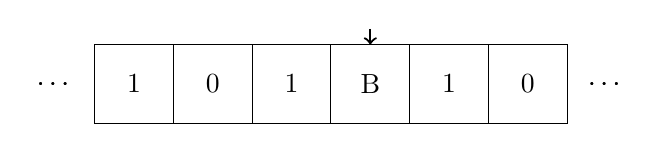
\begin{tikzpicture}
            % Dessiner les cases
            \foreach \x in {-3,-2,-1,0,1,2} {
                \draw (\x,0) rectangle (\x+1,1);
            }
        
            % Ajouter les pointillés aux extrémités
            \node at (-3.5,0.5) {\dots};
            \node at (3.5,0.5) {\dots};
        
            % Ajouter des symboles dans les cases
            \node at (-3.5,0.5) {\dots};
            \node at (-2.5,0.5) {1};
            \node at (-1.5,0.5) {0};
            \node at (-0.5,0.5) {1};
            \node at (0.5,0.5) {B};
            \node at (1.5,0.5) {1};
            \node at (2.5,0.5) {0};
            \node at (3.5,0.5) {\dots};
        
            % Ajouter une tête de lecture
            \draw[thick,->] (0.5,1.2) -- (0.5,1);
        
        \end{tikzpicture}
    \end{center}

    Les machines de Turing constituent une abstraction des ordinateurs tels qu'on les connaît aujourd'hui. Voir Fig 105. On peut aussi se limiter à une demi-droite en guise de bande.
\end{remarque}

\begin{definition}{}{Machine de Turing}
    Une machine de turing est la donnée d'un 7-uplet $\mc{M} = (\Sigma, \Gamma, Q, q_0, F, T, \#)$, où~:
    \begin{itemize}
        \item $\Sigma$ est l'\notion{alphabet d'entrée}. C'est l'ensemble fini des lettres que l'on utilise pour écrire le mot donné en entrée à $\mc{M}$.
        \begin{center}
            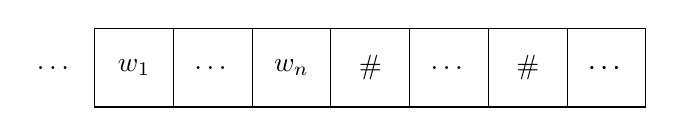
\begin{tikzpicture}
                % Dessiner les cases
                \foreach \x in {-3,-2,-1,0,1,2,3} {
                    \draw (\x,0) rectangle (\x+1,1);
                }
            
                % Ajouter les pointillés aux extrémités
                \node at (-3.5,0.5) {\dots};
                \node at (3.5,0.5) {\dots};
            
                % Ajouter des symboles dans les cases
                % \node at (-3.5,0.5) {\#};
                \node at (-2.5,0.5) {$w_1$};
                \node at (-1.5,0.5) {\dots};
                \node at (-0.5,0.5) {$w_n$};
                \node at (0.5,0.5) {\#};
                \node at (1.5,0.5) {\dots};
                \node at (2.5,0.5) {\#};
                \node at (3.5,0.5) {\dots};
            \end{tikzpicture}
        \end{center}
        $w = w_1 \dots w_n \in \Sigma^*$ est l'entrée donnée. On a ici représenté la configuration initiale de la bande pour cette entrée.
        \item $\#$ est le \notion{symbole blanc}, il sert à remplir les cases non occupées de la bande.
        \item $\Gamma$ est l'\notion{alphabet de bande}. Il est fini, et on a~:
        $$\Sigma \cup \{\#\} \subset \Gamma$$
        \item $Q$ est un \notion{ensemble fini d'états}
        \item $q_0 \in Q$ est l'\notion{état initial}.
        \item $F \subset Q$ est l'\notion{ensemble des états finaux}.
        \item $T$ est l'\notion{ensemble des transitions}. Il vérifie~:
        $$T \subset Q \times \Gamma \times Q \times \Gamma \times \{\triangleleft, \triangleright \}$$
        Une transition est alors~:
        \begin{itemize}
            \item soit de la forme $(q_1, a) \rightarrow (q_2, b, \triangleright)$, auquel cas on est dans l'état $q_1$, on lit $a$, on remplace $a$ par $b$ dans la bande, puis on avance d'une case vers la droite, et on se place en l'état $q_2$.
            \item soit de la forme $(q_1, a) \rightarrow (q_2, b, \triangleleft)$, symétriquement.
        \end{itemize}
    \end{itemize}
\end{definition}

\begin{exemple}{}{de machine de Turing}
    Voir Fig.106
    
\end{exemple}

\begin{remarque}{}{concernant les machines de Turing}
    La bande est infinie à droite. Lors d'un calcul le nombre de cases occupées (cases sans symbole blanc) peut croître indéfiniment et on peut de fait avoir des calculs infinis. Pour autant, on ne peut pas avoir un nombre infini de cases occupées.
\end{remarque}

\begin{definition}{}{configuration d'une machine de Turing}
    On appelle \notion{configuration d'une machine de Turing} est la donnée de l'état d'une machine de Turing~:
    \begin{itemize}
        \item l'état actuel, appelé \notion{état de contrôle}
        \item le contenu de la bande
        \item la position de la tête de lecture
    \end{itemize}
    On note une $C = (u,q,z) = u\,q\,v$ une telle configuration, où~:
    \begin{itemize}
        \item $u$ est le contenu de la bande strictement avant la tête de lecture
        \item $q$ est l'état courant
        \item $v$ est le contenu de la bande après la tête de lecture jusqu'à la dernière case occupée incluse. (tous les symboles blancs suivant sont omis)
    \end{itemize}
\end{definition}

\begin{exemple}{}{de configuration dans une machine de Turing}
    Pour la machine de Turing suivante, Voir fig.107, la configuration représentée est $abca \, q_1 \, \#a $
\end{exemple}

\begin{definition}{}{configuration initale dans une machine de Turing}
    La \notion{configuration initale} dans une machine de Turing lorsqu'on lit un mot $w$ sur une machine de Turing $\mc{M}$ est~:
    $$q_0\, w = (\epsilon, q_0, w)$$
\end{definition}

\begin{definition}{}{étape de calcul dans une machine de Turing}
    Une \notion{étape de calcul} dans une machine de Turing est un couple $(C,C')$ de configurations, noté $C \rightarrow C'$ telle que~:
    \begin{itemize}
        \item Soit on a $C = uc\,q\,av$ et $C' = u\, q'\, cbv$  et $(q,a) \rightarrow (q',b,\triangleleft)$ est une transition, avec~:
        \begin{itemize}
            \item $u,v \in \Gamma^*$
            \item $q,q' \in Q$ 
            \item $a,b,c \in \Gamma$
        \end{itemize}
        \item Soit on a $C = u\,q\,av$ et $C' = ub\, q'\, v$  et $(q,a) \rightarrow (q',b,\triangleright)$ est une transition, avec~:
        \begin{itemize}
            \item $u,v \in \Gamma^*$
            \item $q,q' \in Q$ 
            \item $a,b \in \Gamma$
        \end{itemize}
    \end{itemize}
    Là encore, on appelle \notion{calcul} une suite d'étapes de calcul~:
    $$C_1 \to \dots \to C_n$$
\end{definition}

\begin{definition}{}{calcul acceptant dans une machine de Turing}
    Un \notion{calcul $C_1 \to \dots \to C_n$ acceptant} dans une machine de Turingv vérifie~:
    \begin{itemize}
        \item $C_0 = q_0\,w$ une configuration initiale
        \item $C_k = u\,q\,v$ avec $q \in F$
    \end{itemize}
    On dit que \notion{$\mc{M}$ accepte $w$} (et non plus "reconnaît").
    On note $\mc{L}(\mc{M})$ le langage des mots reconnus par $\mc{M}$
\end{definition}

\begin{remarque}{}{concernant les calculs acceptants}
    Si le calcul est amené à sortie de la bande par la gauche (dans la convention où cette bande est une demi-droite), on dit que \notion{le calcule échoue}.
\end{remarque}

\begin{exemple}{}{de calcul sur une machine de Turing}
    En reprenant la précédente machine de Turing, lisant mot $w = a^8$~:
    \begin{align*}
        &q_0\,aaaaaaaa \\
        \rightarrow & \#\, q_1\, aaaaaaa \\
        \rightarrow & \#a\, q_2\, aaaaaa \\
        \rightarrow & \#aA\, q_3\, aaaaa \\
        \rightarrow & \#aAa\, q_2\, aaaa  \\
        \rightarrow & \#aAaA\, q_3\, aaa \\
        \rightarrow & \#aAaAa\, q_2\, aa  \\
        \rightarrow & \#aAaAaA\, q_3\, a \\
        \rightarrow & \#aAaAaAa\, q_2 \\
        \rightarrow & \#aAaAaA\, q_3\, a  \\
        \rightarrow^* & q_4\, aAaAaAa \\
        \rightarrow & \#\,q_0\, aAaAaAa \\
        \rightarrow & \#\#\, q_1\, AaAaAa \\
        \rightarrow & \#\# A\, q_1 \, aAaAa \\
        \rightarrow & \#\#Aa\, q_2\, AaAa\\\\
        \rightarrow^* \#\#A\#AAA\#\#\, q_5
    \end{align*}
    Le mot est accepté car le cacul termine. (le tableau deux n'a pas été copié).\\
    On peut montrer que $\mc{L}(\mc{M}) = \{a^{2^n},\,  n\in \N\}$. L'idée est que l'on réalise un "tour"~:
    $$q_0 \to q_1 \to \begin{cases*}
        q_2\\ q_3
    \end{cases*} \to q_4 \to q_0$$
    pour elever la moitié des $a$ jusqu'à en avoir un unique.\\
    Si on a un nombre impaire de $a$, on échoue en $q_3$ devant un symbole blanc.
\end{exemple}

\begin{definition}{}{Machine de Turing déterministe}
    Une machine de Turing est \notion{déterministe} lorsque~:
    $$\forall (q,a) \in Q \times \Gamma,\, \abs{\{(q,a,q',c,x) \in T,\, (q',c,x) \in Q\times F\times\{\triangleleft,\, \triangleright\}\}} \leq 1$$
\end{definition}

\begin{remarque}{}{variantes de machines de Turing}
    Il existe plusieurs variantes de machines de Turing~:
    \begin{itemize}
        \item plusieurs bandes
        \item bi-infinie
    \end{itemize}
    mais leur puissance de calcul est la même.
\end{remarque}
\begin{definition}{}{langage récursivement énumérable}
    Un langage $L$ sur un alphabet $\Sigma$ est dit \notion{récursivement énumérable} lorsqu'il existe une machine de Turing $\mc{M}$ telle que $L = \mc{L}(\mc{M})$
\end{definition}

\begin{definition}{}{}
    Soit $\pbm$ un problème de décision, défini par un ensemble $I$ d'instances et une fonction $f: I \to \{vrai, Faux\}$ de prédicat. On peut associer un $\pbm$ un langage.\\
    Pour $i \in I$ une instance de problème, on note $<i>$ un encodage de $i$ (on suppose que l'encodage est unique à toute instance).\\
    On note $\mc{L}_{\pbm} = \{<i>,\, i \in I,\, f(i) = Vrai\}$. C'est le langage des instances positives.
\end{definition}

\begin{remarque}{}{}
    Por résoudre un problème $\pbm$, on peut utiliser une machine de Turing $\mc{M}$ telle que $\mc{L}(\mc{M}) = \mc{L}_\pbm$
\end{remarque}

\begin{exemple}{}{d'encodages}
    Pour les arbres : $\Sigma = \{N,F,(,)\}$.
    $$N(FN(FF)N(N(FF)F))$$
    est un encodage de l'arbre~:
    \begin{center}
        \begin{forest}
            [N[FN[FF]N[N[FF]F]]]
        \end{forest}
    \end{center}
    Pour les entiers, $\Sigma = \{0,1\}$ : écriture en base $2$.
    Pour les graphes, nombre de sommets et liste d'arêtes ($\Sigma = \{0,1,(,),|\}$).
    $$((11)|((0|1)|(1|10)))$$
    est un encodage de : Voir fig.108
\end{exemple}

\begin{definition}{}{problème récursivement énumérable}
    Un problème de décision $\pbm$ tel que $\mc{L}_\pbm$ est récursivmeent énumérable est dit \notion{récursivement énumérable}~: cela correspond aux problèmes \notion{semi-décidables}. Pour une instance positive, on a un calcul fini qui permet de savoir que l'instance est positive.\\
    Pour une instance négative, on peut avoir des calculs infinis~: cela ne permet donc pas de conclure.
\end{definition}

\begin{definition}{}{langage décidable}
    Un langage $L$ écrit sur un alphabet $\Sigma$ est dit \notion{décidable} lorsqu'il existe une machine de Turing sans calcul infini acceptant $L$.\\
    On dit alors que la machine \notion{décide le langage $L$}
\end{definition}

\begin{proposition}{}{équivalence entre deux notions}
    Poour $\pbm$ un problème de décision~:
    $$\mc{L}_\pbm \Longleftrightarrow \mc{P} \text{ décidable}$$
    On appelle aussi ces langages des \notion{langages récursifs}.
\end{proposition}

\begin{proposition}{}{}
    Si un langage $L$ est tel que~:
    \begin{itemize}
        \item $L$ est récursivement énumérable
        \item $\Sigma^* \setminus L$ est récursivement énumérable
    \end{itemize}
    Alors $L$ est récursif.
\end{proposition}

\begin{remarque}{}{}
    C'est analogue au fait que si $\pbm$ et $co\pbm$ sont semi-décidables, alors $\mc{P}$ est décidable.
\end{remarque}

\begin{definition}{}{encodage d'une machine de Turing}
    Soit $\mc{M}$ une machine de Turing, $w \in \Sigma^*$. On note~:
    \begin{itemize}
        \item $<\mc{M}>$ l'encodage de $\mc{M}$
        \item $<w>$ l'encodage de $w$
        \item $<\mc{M}, w>$ l'encdage de $\mc{M}, w$~:
        $$<\mc{M, w}> = <\mc{M}>\$<w>$$
        où $\$$ est un symbole séparateur tiers.
    \end{itemize}
    On note~:
    $$L_\in = \{<\mc{M},w>,\, w \in \mc{L}(\mc{M}),\, \mc{M} \text{ est une machine de Turing et }  w \in \Sigma^*\}$$
    $L_\in$ est appelé \notion{langage d'acceptation}. C'est un \notion{langage récursivement énumérable} (ADMIS).\\\\
\end{definition}

\begin{definition}{}{machine de Turing universelle}
    Une machine de Turing $\mc{M}_u$ telle que $\mc{L}(\mc{M}_u) = \mc{L}_\in$ existe : on l'appelle \notion{machine universelle}.
\end{definition}

\begin{remarque}{}{}
    Le problème~:
    \begin{itemize}
        \item \textbf{Instance}~: $\mc{M}$ machine de Turing, $w \in \Sigma^*$ 
        \item \textbf{Question}~: Est-ce que $\mc{M}$ accepte $w$ ?
    \end{itemize}
    est un problème semi-décidable. Il est indécidable. Donc $L_\in$ n'est pas récursif. On montre cela comme pour le problème de l'arrêt mais avec des calculs des machines de Turing.\\\\
    L'existence d'une machine universelle $\mc{M}_u$ telle que $\mc{L}(\mc{M}_u) = \mc{L}_\in$ vient du fait que l'on peut simuler le calcul de $\mc{M}$ sur $w$ à partir de $<\mc{M}, w>$
\end{remarque}

\begin{definition}{}{mach}
    Soit fonction $f: \Sigma^* \to \Gamma^*$ avec $\Sigma$ et $\Gamma$ deux alphabets finis et $\Sigma \subset \Gamma$. \notion{$f$ est calculable} lorsqu'il existe une machine de Turing $\mc{M}$ qui pour toute entrée $w \in \Sigma^*$ admet un unique calcul acceptant qui s'arrête avec exactement $f(w)$ sur la bande.
\end{definition}

\begin{definition}{}{réduction Turing}
    Soit $A$ et $B$ deux problèmes de décision et $L_A$ et $L_B$ les langages associés d'alphabets de supports $\Sigma_A$ et $\Sigma_B$. Une \notion{réduction Turing} de $A$ vers $B$ (notée $A \leq_T B$) correspond à une fonction $f : \Sigma_A^* \to \Sigma_B^*$ calculable qui permet de transformer une instance du problème $A$ en une instance du problème $B$ telle que~:
    $$w \in L_A \longleftrightarrow f(w) \in L_B$$
\end{definition}


\begin{remarque}{}{idée}
    L'idée est que la machine qui calcule $f$ permet de passer d'une configuration $q_0 \, w$ à une configuration $q_0' \, f(w)$. Ensuite, on peut utiliser si elle existe, la machine $\mc{M}_B$ telle que $\mc{L}(\mc{M}) = L_B$ pour savoir si $f(w) = L_B$, donc si $w \in L_A$.
\end{remarque}

\begin{definition}{}{propriété non triviale}
    Une propriété non triviale est une propriété $\pbm$ telle que~:
    \begin{itemize}
        \item il existe $L$ récursivement énumérable qui vérifie $\mc{P}$
        \item et il existe $L$ récursivement énumérable qui ne vérifie pas $\pbm$.
    \end{itemize}
\end{definition}

\begin{theoreme}{}{de Rice}
    Pour toute propriété \notion{non triviale} $\pbm$ sur les langages récursivement énumérabbles, le problème de savoir si le langage $\mc{L}(\mc{M})$ accepté par une machine $\mc{M}$ vérifie $\pbm$ est indécidable.
\end{theoreme}

\begin{demonstration}
    Soit $\pbm$ une propriété non triviale sur les langages récursivement énumérables.\\
    On a au moins~:
    \begin{itemize}
        \item $L_1$ récursivement énumérable qui vérifie $\mc{P}$
        \item $L_2$ récursivement énumérable qui ne vérifie pas $\mc{P}$
    \end{itemize}
    On pose $L_\pbm = \{<\mc{M}>,\, \mc{L}(\mc{M}) \text{ vérifie } \mc{P}\}$. Montrons que $L_\pbm$ n'est pas un langage décidable en utilisant une réduction faisant intervenir $L_\in$ qui est lui-même indécidable.\\\\
    On peut écrire $L_\in \leq_T L_\pbm$ pour la réduction Turing concernant les problèmes associés aux langages.\\
    Quitte à considérer $co\pbm$, on peut supposer sans perte de généralité que $\varnothing$ ne vérifie pas $\pbm$. Donc $L_1 \neq \varnothing$. On pose $\mc{M}_1$ une machine de Turing telle que $\mc{L}(\mc{M}_1) = L_1$.\\
    Soit $\mc{M},w$ une instance du problème associée à $L_\in$. ON construit une machine $\mc{M}_w$ qui simule l'algorithme suivant~:
    \begin{lstLNAT}
    $M_w$($u \in \Sigma^*$):
        SI $\mc{M}$ accepte $w$:
            Calculer $u$ sur $\mc{M}_1$ (quitte à calculer, rejeter, échouer, ne pas terminer)
        SINON:
            Rejeter
    \end{lstLNAT}
    On admet que l'on peut construire $\mc{M}_w$ à partir de $\mc{M}$, $w$ et $\mc{M}_1$. Montrons que~:
    $$<\mc{M},w> \in L_\in \longleftrightarrow <\mc{M}_w> = L_\pbm$$
    \begin{itemize}
        \item $\boxed{\implies}$ : Si $<\mc{M},w> \in L_\in$, \ie $\mc{M}$ acceptant, on a $\mc{L}(\mc{M}_w) = L_1$, car on est toujours dans le premier cas de l'algorithme. Or $L_1$ vérifie $\pbm$, donc $<\mc{M}_w> \in L_\pbm$.
        \item $\boxed{\impliedby}$ : par contraposée.\\
        Si $<\mc{M},w> \notin L_\in$, \ie $\mc{M}$ n'accepte pas $w$~:
        \begin{itemize}
            \item si le calcul de $\mc{M}$ sur $w$ ne termine pas, pour tout $u$, $\mc{M}_w$ ne termine pas, car vérifier si $\mc{M}$ accepte $w$ ne termine pas donc $\mc{L}(\mc{M}_w) = \varnothing$
            \item Si $\mc{M}$ rejette $w$, on va dans le "sinon" dans tous lescas et tout mot $u$ est rejeté donc $\mc{L}(\mc{M}_w) = \varnothing$
        \end{itemize}
        Or $\varnothing$ ne vérifie pas $\pbm$ donc $<\mc{M}_w> \notin L_\pbm$
    \end{itemize}
\end{demonstration}

\begin{definition}{}{complexité, la vraie}
    Soit $\mc{M}$ une machine de Turing et $\gamma : C_0 \to \dots C_k$ un calcul sur une entrée $w \in \Sigma^*$.\\
    Le \notion{temps de clacul} du calcul $\gamma$ est~:
    $$t_\mc{M}(\gamma) = k$$
    L'espace utilisé par le calcul est~:
    $$s_\mc{M}(\gamma) = \max_{0\leq i \leq k} \abs{C_i}$$
    Pour une entrée $w$, la \notion{complexité temporelle} est définie comme~:
    $$t_\mc{M}(w) = \min_{\gamma \text{ calcul de $w$ sur $\mc{M}$}} \Big(t_\mc{M}(\gamma)\Big)$$
    la \notion{complexité spatiale} est définie par~:
    $$s_\mc{M}(w) = \min_{\gamma \text{ calcul de $w$ sur $\mc{M}$}} \Big(s_\mc{M}(\gamma)\Big)$$
\end{definition}

\begin{remarque}{}{}
    On peut définir pour une machine de Turing $\mc{M}$, pour tout $n \in \N$~:
    $$t_\mc{M}(n) = \max_{\abs{w} = n}\Big(t_\mc{M}(w)\Big)$$
    et~:
    $$s_\mc{M}(n) = \max_{\abs{w} = n}\Big(s_\mc{M}(w)\Big)$$
\end{remarque}

\begin{definition}{}{classes de complexité}
    Soit $f : \N \to \R_+$ (souvent $\N$).
    \begin{enumeratebf}
        \item $TIME(f(n))$ est l'ensemble des problèmes de décision résolus par une machine de Turing déterministe telle que~:
         $$t_\mc{M}(n) = \mc{O}\Big(f(n)\Big)$$
        \item $NTIME(f(n))$ est l'ensemble des problèmes de décision résolus par une machine de Turing non déterministe telle que~:
        $$t_\mc{M}(n) = \mc{O}\Big(f(n)\Big)$$
        \item On a toujours $TIME(f(n)) \subset NTIME(f(n))$.\\
        $$P = \Bigcup_{k \geq 0}TIME(n^k)$$
        $$NP = \Bigcup_{k \geq 0}NTIME(n^k)$$
        $$EXP = EXPTIME = \bigcup_{k \geq 0} TIME(2^{n^k})$$
        $$NEXP = NEXPTIME = \bigcup_{k \geq 0} NTIME(2^{n^k})$$
    \end{enumeratebf} 
\end{definition}

\begin{proposition}{}{machine de Turing}
    Pour toute machine de Turing $\mc{M}$ non déterministe, il existe une machine $\mc{M}'$ déterministe tell que~:
    $$t_{\mc{M}'}(n) = \mc{O}(t_\mc{M}(n)2^{t_\mc{M}(n)})$$
\end{proposition}

\begin{remarque}{}{}
    En pratique, c'est pour cela que les problèmes NP-complets sont résolus en temps EXP.
\end{remarque}

\begin{proposition}{}{}
    $P \subset NP \subset EXP \subset NEXP$.
\end{proposition}



\end{document}